\chapter{次のブロックへ切り替える}
\section{ブロックが一番下まで落ちた時とは}
ブロックがこれ以上下に落ちられないとき、次のブロックに切り替える処理を書きます。
現在、1秒に一回、ブロックが落ちるようになっているので、そこを利用しましょう。
\begin{figure}[h]
  \centering
  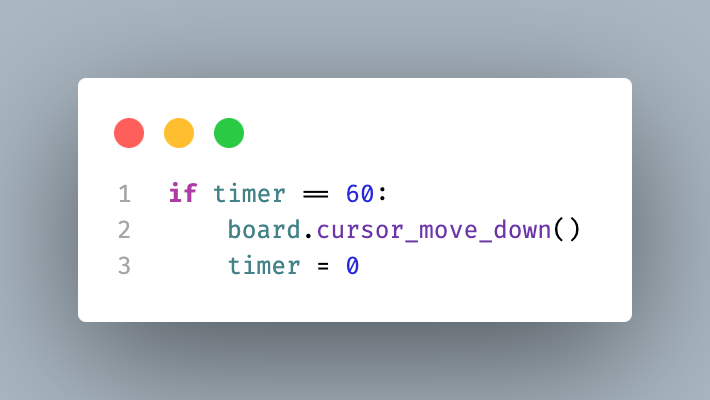
\includegraphics[width=100mm]{images/timer.png}
  \caption{「一秒経った時」を実現しているif文}
\end{figure}

\subsection{Boardクラスに新しい関数updateを追加}
Boardクラスに新しい関数updateを追加します。
mainに「もしブロックが…」のような処理を書いても動きはするのですが、
役割分担の考え方からBoardクラスに書くことにします。
\lstinputlisting[caption={定期的にブロックを落とし、落とせないなら次のブロックを用意するupdate関数}, language=Python]{chapter10/ch10_1_1.py}
次に、main関数を変更します。今まで単純にブロックを落としていた部分をupdate関数に変更します。
\lstinputlisting[caption={main関数を変更する}, language=Python]{chapter10/ch10_1_2.py}
実行すると、ブロックが一番下まで落ちたら次のブロックに切り替わるようになります。

\section{ブロックを積む}
前回のセクションでは、ブロックが切り替わった時に前のブロックが消えてしまう問題がありました。
今回は、ブロックが一番下まで落ちた時に、そのブロックを置く処理を書きます。
\subsection{Boardクラスにfix関数を追加}
Boardクラスにfix関数を追加します\footnote{fix: 固定する、直す}。
ここで、盤面がどのように描かれているかを復習します。
\subsubsection{スクリーンへの書き込みを行なっている場所}
実際にウィンドウへの書き込みを行なっているのは、draw関数です。
その中でも、\textbf{2~5行目が盤面の描画}、7~9行目がカーソルを灰色にする処理、
14~36行目が現在持っているブロックの描画、42~45行目が枠線の描画になっています。
\begin{figure}
  [h]
  \centering
  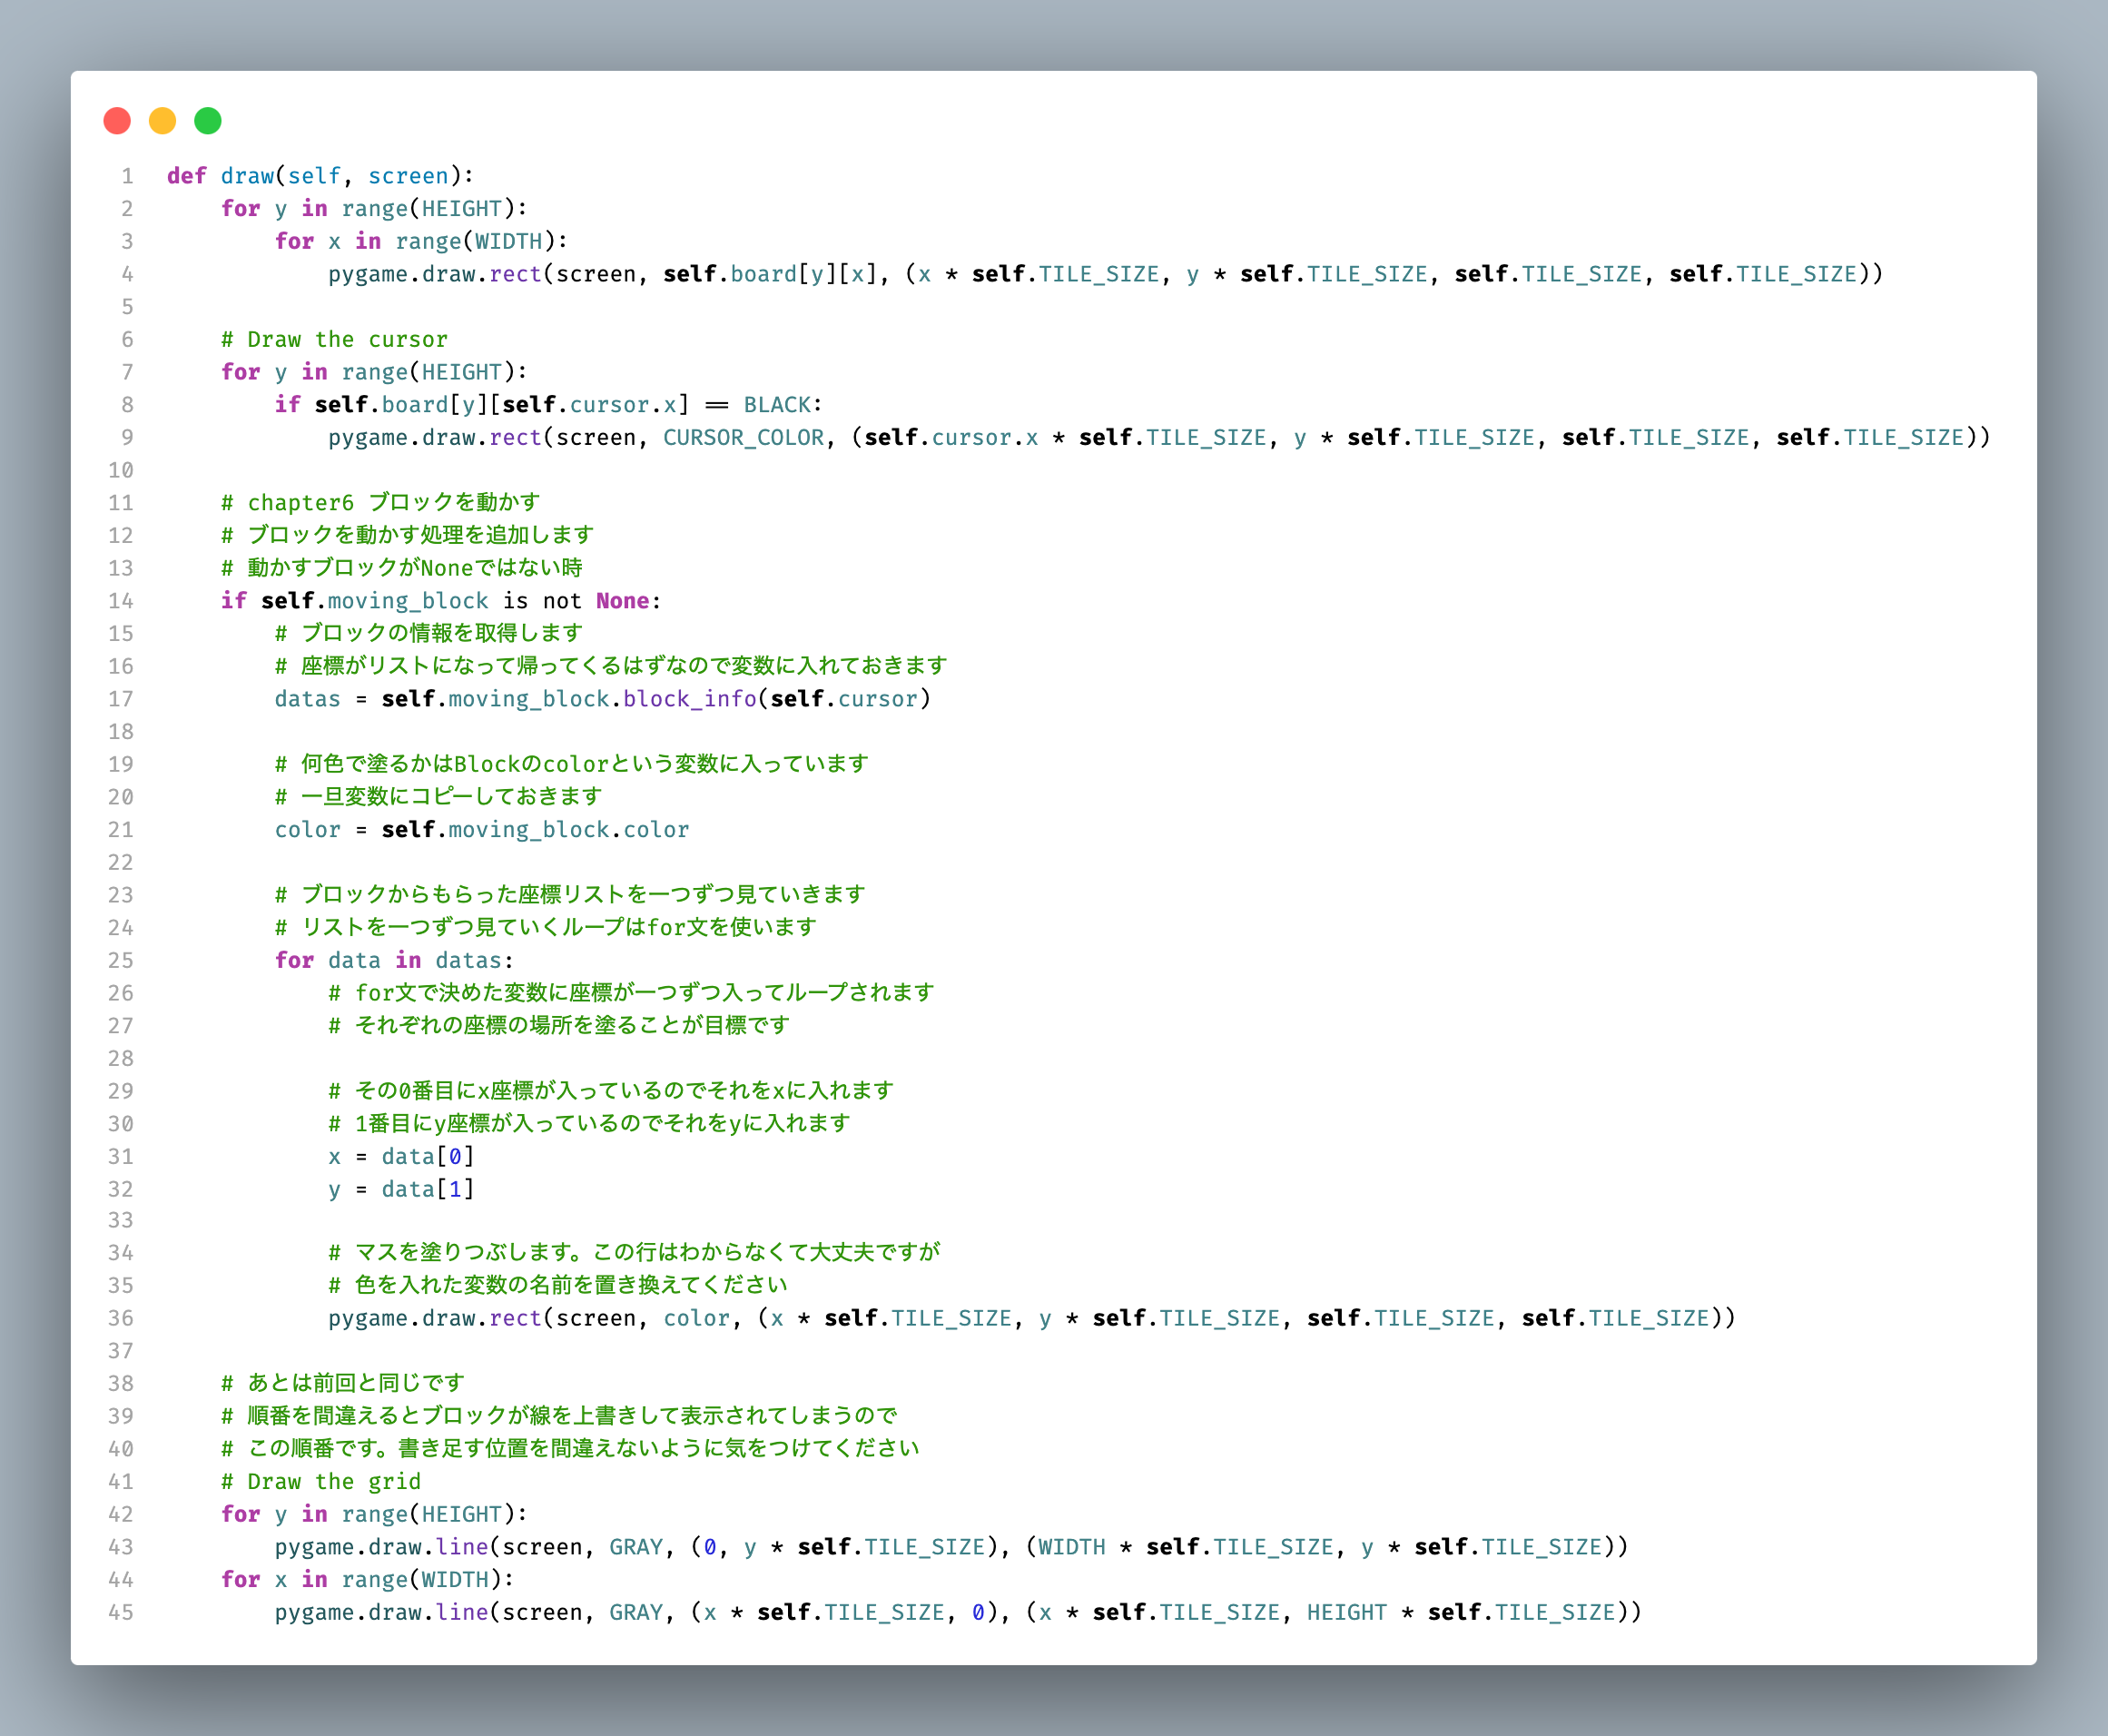
\includegraphics[width=100mm]{images/DrawFunction.png}
  \caption{draw関数の中身}
\end{figure}
ここから、self.boardの中身を変更すれば、draw関数が自動的に画面に反映してくれそうです。
\begin{figure}
  [h]
  \centering
  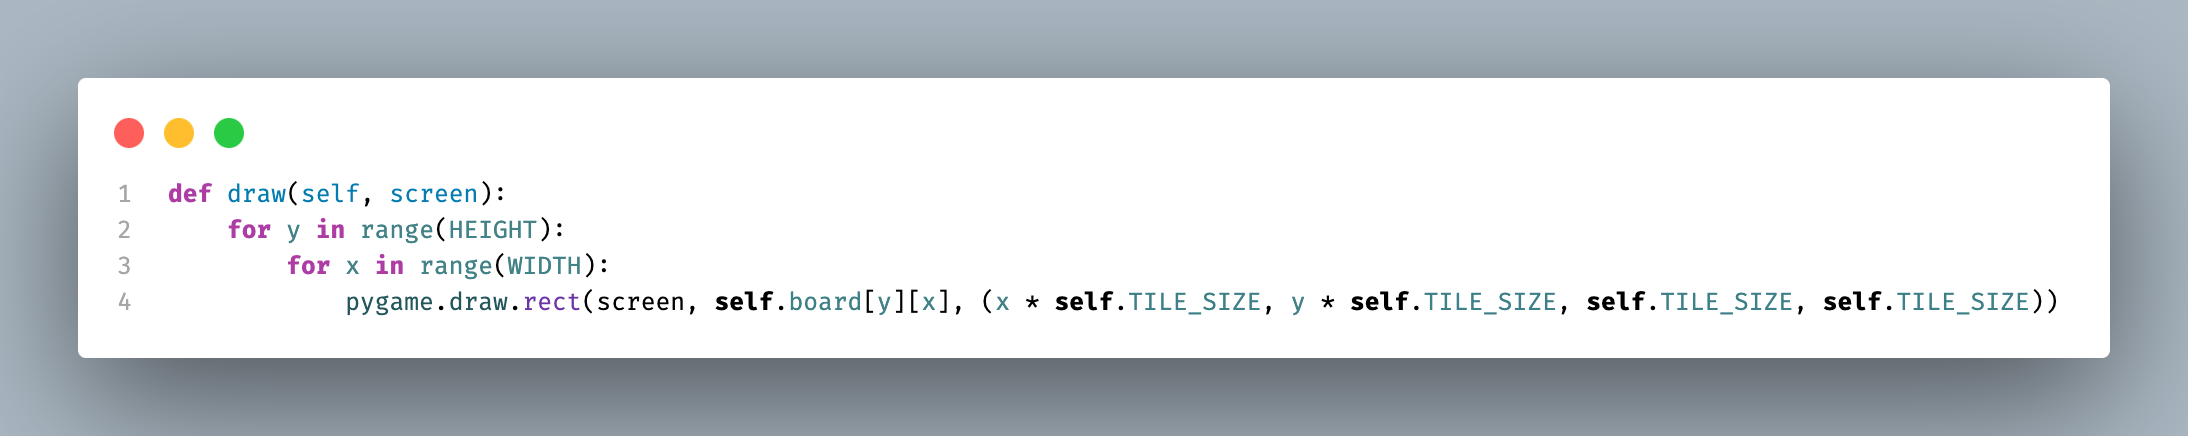
\includegraphics[width=\textwidth]{images/DrawBoard.png}
  \caption{self.boardを変更すれば画面にも反映されそう}
\end{figure}

\subsection{fix関数を実装}
fix関数を実装します。
\lstinputlisting[caption={fix関数}, language=Python]{chapter10/ch10_2_1.py}
次に、update関数を変更します。
\lstinputlisting[caption={update関数を変更}, language=Python]{chapter10/ch10_2_2.py}
実行すると、ブロックが一番下まで落ちたら、そのブロックが盤面に固定されるようになります。